\documentclass[]{book}
\usepackage{lmodern}
\usepackage{amssymb,amsmath}
\usepackage{ifxetex,ifluatex}
\usepackage{fixltx2e} % provides \textsubscript
\ifnum 0\ifxetex 1\fi\ifluatex 1\fi=0 % if pdftex
  \usepackage[T1]{fontenc}
  \usepackage[utf8]{inputenc}
\else % if luatex or xelatex
  \ifxetex
    \usepackage{mathspec}
  \else
    \usepackage{fontspec}
  \fi
  \defaultfontfeatures{Ligatures=TeX,Scale=MatchLowercase}
\fi
% use upquote if available, for straight quotes in verbatim environments
\IfFileExists{upquote.sty}{\usepackage{upquote}}{}
% use microtype if available
\IfFileExists{microtype.sty}{%
\usepackage{microtype}
\UseMicrotypeSet[protrusion]{basicmath} % disable protrusion for tt fonts
}{}
\usepackage[margin=1in]{geometry}
\usepackage{hyperref}
\hypersetup{unicode=true,
            pdftitle={A Second Semester Statistics Course with R},
            pdfauthor={Mark Greenwood and Katherine Banner},
            pdfborder={0 0 0},
            breaklinks=true}
\urlstyle{same}  % don't use monospace font for urls
\usepackage{natbib}
\bibliographystyle{apalike}
\usepackage{color}
\usepackage{fancyvrb}
\newcommand{\VerbBar}{|}
\newcommand{\VERB}{\Verb[commandchars=\\\{\}]}
\DefineVerbatimEnvironment{Highlighting}{Verbatim}{commandchars=\\\{\}}
% Add ',fontsize=\small' for more characters per line
\usepackage{framed}
\definecolor{shadecolor}{RGB}{248,248,248}
\newenvironment{Shaded}{\begin{snugshade}}{\end{snugshade}}
\newcommand{\KeywordTok}[1]{\textcolor[rgb]{0.13,0.29,0.53}{\textbf{{#1}}}}
\newcommand{\DataTypeTok}[1]{\textcolor[rgb]{0.13,0.29,0.53}{{#1}}}
\newcommand{\DecValTok}[1]{\textcolor[rgb]{0.00,0.00,0.81}{{#1}}}
\newcommand{\BaseNTok}[1]{\textcolor[rgb]{0.00,0.00,0.81}{{#1}}}
\newcommand{\FloatTok}[1]{\textcolor[rgb]{0.00,0.00,0.81}{{#1}}}
\newcommand{\ConstantTok}[1]{\textcolor[rgb]{0.00,0.00,0.00}{{#1}}}
\newcommand{\CharTok}[1]{\textcolor[rgb]{0.31,0.60,0.02}{{#1}}}
\newcommand{\SpecialCharTok}[1]{\textcolor[rgb]{0.00,0.00,0.00}{{#1}}}
\newcommand{\StringTok}[1]{\textcolor[rgb]{0.31,0.60,0.02}{{#1}}}
\newcommand{\VerbatimStringTok}[1]{\textcolor[rgb]{0.31,0.60,0.02}{{#1}}}
\newcommand{\SpecialStringTok}[1]{\textcolor[rgb]{0.31,0.60,0.02}{{#1}}}
\newcommand{\ImportTok}[1]{{#1}}
\newcommand{\CommentTok}[1]{\textcolor[rgb]{0.56,0.35,0.01}{\textit{{#1}}}}
\newcommand{\DocumentationTok}[1]{\textcolor[rgb]{0.56,0.35,0.01}{\textbf{\textit{{#1}}}}}
\newcommand{\AnnotationTok}[1]{\textcolor[rgb]{0.56,0.35,0.01}{\textbf{\textit{{#1}}}}}
\newcommand{\CommentVarTok}[1]{\textcolor[rgb]{0.56,0.35,0.01}{\textbf{\textit{{#1}}}}}
\newcommand{\OtherTok}[1]{\textcolor[rgb]{0.56,0.35,0.01}{{#1}}}
\newcommand{\FunctionTok}[1]{\textcolor[rgb]{0.00,0.00,0.00}{{#1}}}
\newcommand{\VariableTok}[1]{\textcolor[rgb]{0.00,0.00,0.00}{{#1}}}
\newcommand{\ControlFlowTok}[1]{\textcolor[rgb]{0.13,0.29,0.53}{\textbf{{#1}}}}
\newcommand{\OperatorTok}[1]{\textcolor[rgb]{0.81,0.36,0.00}{\textbf{{#1}}}}
\newcommand{\BuiltInTok}[1]{{#1}}
\newcommand{\ExtensionTok}[1]{{#1}}
\newcommand{\PreprocessorTok}[1]{\textcolor[rgb]{0.56,0.35,0.01}{\textit{{#1}}}}
\newcommand{\AttributeTok}[1]{\textcolor[rgb]{0.77,0.63,0.00}{{#1}}}
\newcommand{\RegionMarkerTok}[1]{{#1}}
\newcommand{\InformationTok}[1]{\textcolor[rgb]{0.56,0.35,0.01}{\textbf{\textit{{#1}}}}}
\newcommand{\WarningTok}[1]{\textcolor[rgb]{0.56,0.35,0.01}{\textbf{\textit{{#1}}}}}
\newcommand{\AlertTok}[1]{\textcolor[rgb]{0.94,0.16,0.16}{{#1}}}
\newcommand{\ErrorTok}[1]{\textcolor[rgb]{0.64,0.00,0.00}{\textbf{{#1}}}}
\newcommand{\NormalTok}[1]{{#1}}
\usepackage{longtable,booktabs}
\usepackage{graphicx,grffile}
\makeatletter
\def\maxwidth{\ifdim\Gin@nat@width>\linewidth\linewidth\else\Gin@nat@width\fi}
\def\maxheight{\ifdim\Gin@nat@height>\textheight\textheight\else\Gin@nat@height\fi}
\makeatother
% Scale images if necessary, so that they will not overflow the page
% margins by default, and it is still possible to overwrite the defaults
% using explicit options in \includegraphics[width, height, ...]{}
\setkeys{Gin}{width=\maxwidth,height=\maxheight,keepaspectratio}
\IfFileExists{parskip.sty}{%
\usepackage{parskip}
}{% else
\setlength{\parindent}{0pt}
\setlength{\parskip}{6pt plus 2pt minus 1pt}
}
\setlength{\emergencystretch}{3em}  % prevent overfull lines
\providecommand{\tightlist}{%
  \setlength{\itemsep}{0pt}\setlength{\parskip}{0pt}}
\setcounter{secnumdepth}{5}
% Redefines (sub)paragraphs to behave more like sections
\ifx\paragraph\undefined\else
\let\oldparagraph\paragraph
\renewcommand{\paragraph}[1]{\oldparagraph{#1}\mbox{}}
\fi
\ifx\subparagraph\undefined\else
\let\oldsubparagraph\subparagraph
\renewcommand{\subparagraph}[1]{\oldsubparagraph{#1}\mbox{}}
\fi

%%% Use protect on footnotes to avoid problems with footnotes in titles
\let\rmarkdownfootnote\footnote%
\def\footnote{\protect\rmarkdownfootnote}

%%% Change title format to be more compact
\usepackage{titling}

% Create subtitle command for use in maketitle
\newcommand{\subtitle}[1]{
  \posttitle{
    \begin{center}\large#1\end{center}
    }
}

\setlength{\droptitle}{-2em}
  \title{A Second Semester Statistics Course with R}
  \pretitle{\vspace{\droptitle}\centering\huge}
  \posttitle{\par}
  \author{Mark Greenwood and Katherine Banner}
  \preauthor{\centering\large\emph}
  \postauthor{\par}
  \predate{\centering\large\emph}
  \postdate{\par}
  \date{2017-05-26}

\usepackage{booktabs}

\begin{document}
\maketitle

{
\setcounter{tocdepth}{1}
\tableofcontents
}
\chapter*{Acknowledgments}\label{acknowledgments}
\addcontentsline{toc}{chapter}{Acknowledgments}

\chapter{Preface}\label{preface}

This book is designed primarily for use in a second semester statistics
course although it can also be useful for researchers needing a quick
review or ideas for using R for the methods discussed in the text. As a
text primarily designed for a second statistics course, it presumes that
you have had an introductory statistics course. There are now many
different varieties of introductory statistics from traditional,
formula-based courses (called ``consensus'' curriculum courses) to more
modern, computing-intensity courses that use randomization ideas to try
to enhance learning of basic statistical methods. We are not going to
presume that you have had a particular ``flavor'' of introductory
statistics or that you had your introductory statistics out of a
particular text, just that you have had a course that tried to introduce
you to the basic terminology and ideas underpinning statistical
reasoning. We would expect that you are familiar with the logic (or
sometimes illogic) of hypothesis testing including null and alternative
hypothesis and confidence interval construction and interpretation and
that you have seen all of this in a couple of basic situations. We start
with a review of these ideas in one and two group situations with a
quantitative response, something that you should have seen before.

This text covers a wide array of statistical tools that are connected
through situation, methods used, or both. As we explore various
techniques, look for the identifying characteristics of each method --
what type of research questions are being addressed (relationships or
group differences, for example) and what type of variables are being
analyzed (quantitative or categorical). \textbf{\emph{Quantitative
variables}} are made up of numerical measurements that have meaningful
units attached to them. \textbf{\emph{Categorical variables}} take on
values that are categories or labels. Additionally, you will need to
carefully identify the \textbf{\emph{response}} variables, where the
study and variable characteristics should suggest which variables should
be used as the explanatory variables that may explain variation in the
response variable. Because this is an intermediate statistics course, we
will start to handle more complex situations (many explanatory
variables) and will provide some tools for graphical explorations to
complement the more sophisticated statistical models required to handle
these situations.

\section{Overview of methods}\label{overview-of-methods}

After you are introduced to basic statistical ideas, a wide array of
statistical methods become available. The methods explored here focus on
assessing (estimating and testing for) relationships between variables,
sometimes when controlling for or modifying relationships based on
levels of another variable -- which is where statistics gets interesting
and really useful. Early statistical analyses (approximately 100 years
ago) were focused on describing a single variable. Your introductory
statistics course should have heavily explored methods for summarizing
and doing inference in situations with one group or where you were
comparing results for two groups of observations. Now, we get to
consider more complicated situations -- culminating in a set of tools
for working with multiple explanatory variables, some of which might be
categorical and related to having different groups of subjects that are
being compared. Throughout the methods we will cover, it will be
important to retain a focus on how the appropriate statistical analysis
depends on the research question and data collection process as well as
the types of variables measured.

Figure \ref{fig:Figure1} frames the topics we will discuss. Taking a
broad vision of the methods we will consider, there are basically two
scenarios -- one when the response is quantitative and one when the
response is categorical. Examples of quantitative responses we will see
later involve \emph{suggested jail sentence} (in years) and \emph{body
fat} (percentage). Examples of categorical variables include
\emph{improvement} (none, some, or marked) in a clinical trial or
whether a student has turned in copied work (never, exam or paper, or
both). There are going to be some more nuanced aspects to all these
analyses as the complexity of both sides of Figure \ref{fig:Figure1}
suggest, but note that near the bottom, each tree converges on a single
procedure, using a \textbf{\emph{linear model}} for a quantitative
response variable or using a \textbf{\emph{Chi-square test}} for a
categorical response. After selecting the appropriate procedure and
completing the necessary technical steps to get results for a given data
set, the final step involves assessing the scope of inference and types
of conclusions that are appropriate based on the design of the study.



\begin{figure}
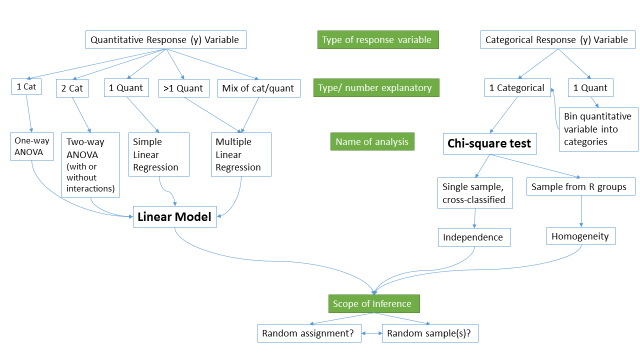
\includegraphics[width=8.89in]{chapter0_files/image001} \caption{Flow chart of methods}\label{fig:Figure1}
\end{figure}

We will be spending most of the semester working on methods for
quantitative response variables (the left side of Figure
\ref{fig:Figure1} covered in Chapters 1, 2, 3, 5, 6, and 7) and stepping
over to handle the situation with a categorical response variable (right
side of Figure \ref{fig:Figure1} that is discussed in Chapter 4).
Chapter 8 contains case studies illustrating all the methods discussed
previously, providing a final opportunity to explore additional examples
that illustrate how finding your way through the paths in Figure
\ref{fig:Figure1} leads to the appropriate analysis.

The first topics (Chapters 0 and 1) will be more familiar as we start
with single and two group situations with a quantitative response. In
your previous statistics course, you should have seen methods for
estimating and quantifying uncertainty for the mean of a single group
and for differences in the means of two groups. Once we have briefly
reviewed these methods and introduced the statistical software that we
will use throughout the course, we will consider the first new
statistical material in Chapter 2. It involves the situation with a
quantitative response variable where there are more than 2 groups to
compare -- this is what we call the \textbf{\emph{One-Way ANOVA}}
situation. It generalizes the 2-independent sample hypothesis test to
handle situations where more than 2 groups are being studied. When we
learn this method, we will begin discussing model assumptions and
methods for assessing those assumptions that will be present in every
analysis involving a quantitative response. The \textbf{\emph{Two-Way
ANOVA}} (Chapter 3) considers situations with two categorical
explanatory variables and a quantitative response. To make this somewhat
concrete, suppose we are interested in assessing differences in, say,
the \emph{yield} of wheat from a field based on the amount of
\emph{fertilizer} applied(none, low, or high) and \emph{variety} of
wheat (two types). Here, \emph{yield} is a quantitative response
variable that might be measured in bushels per acre and there are two
categorical explanatory variables, \emph{fertilizer}, with 3 levels, and
\emph{variety}, with two levels. In this material, we introduce the idea
of an \textbf{\emph{interaction}} between the two explanatory variables:
the relationship between one categorical variable and the mean of the
response changes depending on the levels of the other categorical
variable. For example, extra fertilizer might enhance the growth of one
variety and hinder the growth of another so we would say that
\emph{fertilizer} has different impacts based this interaction may or
may not actually be present, we will consider two versions of the model
in Two-Way ANOVAs, what are called the \textbf{\emph{additive}} (no
interaction) and the \textbf{\emph{interaction}} models.

Following the methods for two categorical variables and a quantitative
response, we explore a method for analyzing data where the response is
categorical, called the \textbf{\emph{Chi-square test}} in Chapter 4.
This most closely matches the One-Way ANOVA situation with a single
categorical explanatory variable, except now the response variable is
categorical. For example, we will assess whether taking a drug (vs
taking a \textbf{\emph{placebo}}\footnote{A \textbf{\emph{placebo}} is a
  treatment level designed to mimic the potentially efficacious level(s)
  but that can have no actual effect. The \textbf{\emph{placebo effect}}
  is the effect that thinking that an effective treatment was received
  has on subjects. There are other related issues in performing
  experiments like the \textbf{\emph{Hawthorne}} or observer
  \textbf{\emph{effect}} where subjects modify behavior because they are
  being observed.}) has an \textbf{\emph{effect}}\footnote{We will
  reserve the term ``effect'' for situations where we could potentially
  infer causal impacts on the response of the explanatory variable which
  occurs in situations where the levels of the explanatory variable are
  randomly assigned to the subjects.} on the type of improvement the
subjects demonstrate. There are two different scenarios for study design
that impact the analysis technique and hypotheses tested in Chapter 4.
If the explanatory variable reflects the group that subjects were
obtained from, either through randomization of the treatment level to
the subjects or by taking samples from separate populations, this is
called a \textbf{\emph{Chi-square Homogeneity Test}}. It is also
possible to obtain a single sample from a population and then obtain
information on the levels of the explanatory variable for each subject.
We will analyze these results using what is called a
\textbf{\emph{Chi-square Independence Test}}. They both use the same
test statistic but we use slightly different graphics and are testing
different hypotheses in these two related situations. Figure
\ref{fig:Figure1} also shows that if we had a quantitative explanatory
variable and a categorical response that we would need to ``bin'' or
create categories of responses from the quantitative variable to use the
Chi-square testing methods.

If the predictor and response variables are both quantitative, we start
with scatterplots, correlation, and \textbf{\emph{simple linear
regression}} models (Chapters 5 and 6) -- things you should have seen,
at least to some degree, previously. The biggest differences here will
be the depth of exploration of diagnostics and inferences for this model
and discussions of transformations of variables. If there is more than
one explanatory variable, then we say that we are doing
\textbf{\emph{multiple linear regression}} (Chapter 7) -- the
``multiple'' part of the name reflects that there will be more than one
explanatory variable. We use the same name if we have a mix of
categorical and quantitative predictor variables but there are some new
issues in setting up the models and interpreting the coefficients that
we need to consider. In the situation with one categorical predictor and
one quantitative predictor, we revisit the idea of an interaction. It
allows us to consider situations where the estimated relationship
between a quantitative predictor and the mean response varies among
different levels of the categorical variable.

By the end of Chapter 8 you should be able to identify, perform using
the statistical software R (R Core Team, 2016), and interpret the
results from each of these methods. There is a lot to learn, but many of
the tools for using R and interpreting results of the analyses
accumulate and repeat during the semester. If you work hard to
understand the initial methods, it will help you when the methods get
more complicated. You will likely feel like you are just starting to
learn how to use R at the end of the semester and for learning a new
language that is actually an accomplishment. We will just be taking you
on the first steps of a potentially long journey and it is up to you to
decide how much further you want to go with learning the software.

All the methods you will learn require you to carefully consider how the
data were collected, how that pertains to the population of interest,
and how that impacts the inferences that can be made. The
\textbf{\emph{scope of inference}} from the bottom of Figure
\ref{fig:Figure1} is our shorthand term for remembering to think about
two aspects of the study -- \textbf{\emph{random assignment}} and
\textbf{\emph{random sampling}} . In a given situation, you need to use
the description of the study to decide if the explanatory variable was
randomly assigned to study units (this allows for \textbf{\emph{causal
inferences}} if differences are detected) or not (so no causal
statements are possible). As an example, think about two studies, one
where students are randomly assigned to either get tutoring with their
statistics course or not and another where the students are asked at the
end of the semester whether they sought out tutoring or not. Suppose we
compare the final grades in the course for the two groups (tutoring/not)
and find a big difference. In the first study with random assignment, we
can say the tutoring caused the differences we observed. In the second,
we could only say that the tutoring was associated with differences but
because students self-selected the group they ended up in, we can't say
that the tutoring caused the differences. The other aspect of scope of
inference concerns random sampling: If the data were obtained using a
random sampling mechanism, then our inferences can be safely extended to
the population that the sample was taken from. However, if we have
non-random sample, our inference can only apply to the sample collected.
In the previous example, the difference would be studying a random
sample of students from the population of, say, Introductory Statistics
students at a university vs studying a sample of students that
volunteered for the research project, maybe for extra credit in the
class. We could still randomly assign them to tutoring/not but the
non-random sample would only lead to conclusions about those students
that volunteered. The most powerful scope of inference is when there are
randomly assigned levels of explanatory variables with a random sample
from population -- conclusions would be about causal impacts that would
happen in the population.

By the end of this material, you should have some basic R skills and
abilities to create basic ANOVA and Regression models, as well as to
handle Chi-squared testing situations. Together, this should prepare you
for future statistics courses or for other situations where you are
expected to be able to identify an appropriate analysis, do the
calculations for a given data set, and then effectively communicate
interpretations for the methods discussed here.

\section{Getting started in R}\label{getting-started-in-r}

You will need to download the statistical software package called R and
an enhanced interface to R called RStudio (RStudio, 2016). They are open
source and free to download and use (and will always be that way). This
means that the skills you learn now can follow you the rest of your
life. R is becoming the primary language of statistics and is being
adopted across academia, government, and businesses to help manage and
learn from the growing volume of data being obtained. Hopefully you will
get a sense of some of the power of R in this book.

The next pages will walk you through the process of getting the software
downloaded and provide you with an initial experience using RStudio to
do things that should look familiar even though the interface will be a
new experience. Do not expect to master R quickly -- it takes years
(sorry!) even if you know the statistical methods being used. We will
try to keep all your interactions with R code in a similar code format
and that should help you in learning how to use R as we move through
various methods. We will also usually provide you with example code.
Everyone that learns R starts with copying other people's code and then
making changes for specific applications -- so expect to go back to
examples from the text and focus on learning how to modify that code to
work for your particular data set. Only really experienced R users
``know'' functions without having to check other resources. After we
complete this basic introduction, Chapter 1 begins doing more
sophisticated things with R, allowing us to compare quantitative
responses from two groups, make some graphical displays, do hypothesis
testing and create confidence intervals in a couple of different ways.

You will have two downloading activities to complete before you can do
anything more than read this book\footnote{I recorded a video that walks
  through the material on the following pages that is available here:
  \url{https://camtasia.msu.montana.edu/Relay/Files/w76c139/RandRstudio_Final/RandRstudio_Final_-_20160715_130555_23.html}
  in the digital version of the book.}. First, you need to download R.
It is the engine that will do all the computing for us, but you will
only interact with it once. Go to \url{http://cran.rstudio.com} and
click on the ``\textbf{Download R for\ldots{}}'' button that corresponds
to your operating system. On the next page, click on ``\textbf{base}''
and then it will take you to a screen to download the most current
version of R that is compiled for your operating system, something like
``\textbf{Download R 3.3.1 for Windows}''. Click on that link and then
open the file you downloaded. You will need to select your preferred
language (choose English so your instructor can help you), then hit
``\textbf{Next}'' until it starts to unpack and install the program (all
the base settings will be fine). After you hit ``\textbf{Finish}'' you
will not do anything further with R directly.

Second, you need to download RStudio. It is an enhanced interface that
will make interacting with R less frustrating. To download RStudio, go
to \url{http://www.rstudio.com/products/rstudio/download/} and select
the correct version under ``Installers for Supported Platforms'' for
your operating system. Download and then install RStudio using the
installer. From this point forward, you should only open RStudio; it
provides your interface with R. Note that both R and RStudio are updated
frequently (up to four times a year) and if you downloaded either more
than a few months previously, you should download the up-to-date
versions, especially if something you are trying to do is not working.
Sometimes code will not work in older versions of R and sometimes old
code won't work in new versions of R.\footnote{The need to keep the code
  up-to-date as R continues to evolve is one reason that this book is
  locally published and that this is the 3\(^{rd}\) version in three
  years\ldots{}}

To get started, we can complete some basic tasks in R using the RStudio
interface. When you open RStudio, you will see a screen like Figure 2.
The added annotation in this and the following screen-grabs is there to
help you get initially oriented to the software interface. R is
command-line software -- meaning that most of the time you have to
create code and then enter and execute it at a command prompt to get any
results. RStudio makes the management and execution of that code more
efficient than the basic version of R. In RStudio, the lower left panel
is called the ``console'' window and is where you can type R code
directly into R or where you will see the code you run and (most
importantly!) where the results of your executed commands will show up.
The most basic interaction with R is available once you get the cursor
active at the command prompt ``\textgreater{}'' by clicking in that
panel (look for a blinking vertical line). The upper left panel is for
writing, saving, and running your R code. Once you have code available
in this window, the ``Run'' button will execute the code for the line
that your cursor is on or for any text that you have highlighted with
your mouse. The ``data management'' or environment panel is in the upper
right, providing information on what data sets have been loaded. It also
contains the ``Import Dataset'' button that provides the easiest way for
you to read a data set into R so you can analyze it. The lower right
panel contains information on the ``Packages'' (additional code we will
download and install to add functionality to R) that are available and
is where you will see plots that you make and requests for ``Help'' on
specific functions.



\begin{figure}
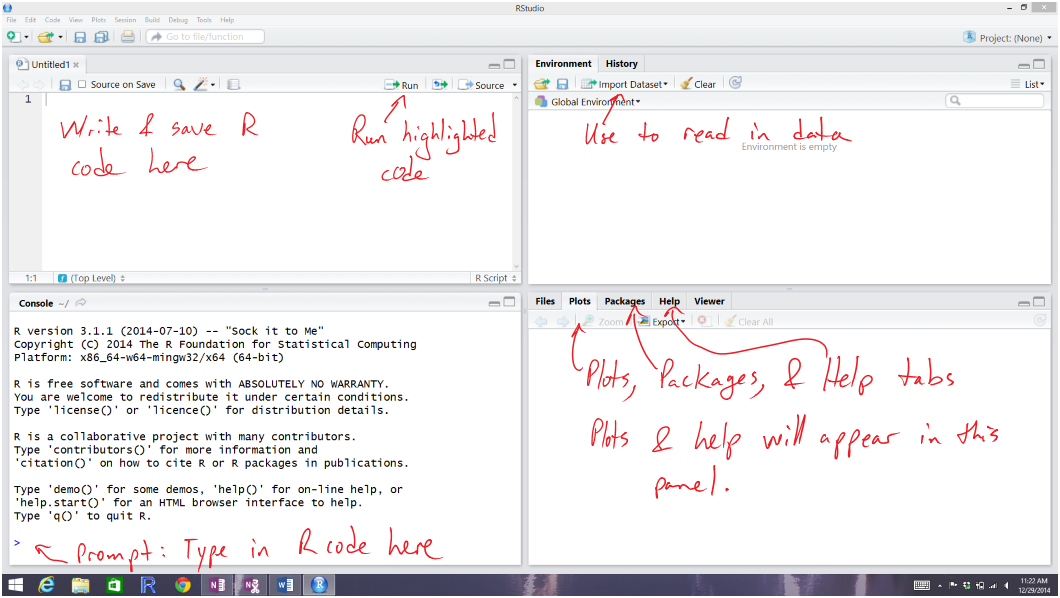
\includegraphics[width=14.72in]{chapter0_files/image003} \caption{Initial RStudio layout}\label{fig:Figure2}
\end{figure}

As a first interaction with R we can use it as a calculator. To do this,
click near the command prompt (\texttt{\textgreater{}}) in the lower
left ``console'' panel, type 3+4, and then hit enter. It should look
like this:

\begin{verbatim}
> 3+4
[1] 7
\end{verbatim}

You can do more interesting calculations, like finding the mean of the
numbers 3, 5, 7, and 8 by adding them up and dividing by 4:

\begin{Shaded}
\begin{Highlighting}[]
\NormalTok{>}\StringTok{ }\NormalTok{(-}\DecValTok{3+5+7+8}\NormalTok{)/}\DecValTok{4}
\NormalTok{[}\DecValTok{1}\NormalTok{] }\DecValTok{4}\NormalTok{. }\DecValTok{25}
\end{Highlighting}
\end{Shaded}

Note that the parentheses help R to figure out your desired order of
operations. If you drop that grouping, you get a very different (and
wrong!) result:

\begin{verbatim}
> -3+5+7+8/4
[1] 11
\end{verbatim}

We could estimate the standard deviation similarly using the formula you
might remember from introductory statistics, but that will only work in
very limited situations. To use the real power of R this semester, we
need to work with data sets that store the Basically, we need to store
observations in named vectors (one dimensional arrays) that contain a
list of the observations. To create a vector containing the four numbers
and assign it to a variable named \emph{variable1}, we need to create a
vector using the function \texttt{c} which means ``combine the items''
that follow, if they are inside parentheses and have commas separating
the values, as follows:

\begin{verbatim}
> c(-3, 5, 7, 8)
[1] -3 5 7 8
\end{verbatim}

To get this vector stored in a variable called \emph{variable1} we need
to use the assignment operator, \texttt{\textless{}-} (read as ``stored
as'') that assigns the information on the right into the variable that
you are creating on the left.

\begin{verbatim}
> variable1 <- c(-3, 5, 7, 8)
\end{verbatim}

In R, the assignment operator, \texttt{\textless{}-}, is created by
typing a ``less than'' symbol \texttt{\textless{}} followed by a
``minus'' sign (\texttt{-}) ever want to see what numbers are residing
in an object in R, just type its name and hit \emph{enter}. You can see
how that variable contains the same information that was initially
generated by \texttt{c(-3,\ 5,\ 7,\ 8)} but is easier to access since we
just need the text for the variable name representing that vector.

\begin{verbatim}
> variable1
[1] -3 5 7 8
\end{verbatim}

With the data stored in a variable, wean use functions such as
\texttt{mean} and \texttt{sd} to find the mean and standard deviation of
the observations contained in \texttt{variable1} :

\begin{verbatim}
> mean(variable1)
[1] 4.25
> sd(variable1)
[1] 4.99166
\end{verbatim}

When dealing with real data, we will often have information about more
than one variable. We could enter all observations by hand for each
variable but this is prone to error and onerous for all but the smallest
data sets. If you are to ever utilize the power of statistics in the
evolving data-centered world, data management has to be accomplished in
a more sophisticated way. While you can manage data sets quite
effectively in R, it is often easiest to start with your data set in
something like Microsoft Excel or OpenOffice's Calc. You want to make
sure that observations are in the rows and the names of variables are in
the columns and that there is no ``extra stuff'' in the spreadsheet. If
you have missing observations, they should be represented with blank
cells. The file should be saved as a ``.csv'' file (stands for
comma-separated values although Excel calls it ``CSV (Comma
Delimited)'', which basically strips off some of the junk that Excel
adds to the necessary information in the file. Excel will tell you that
this is a bad idea, but it actually creates a more stable archival
format and one that R can use directly\footnote{There are ways to read
  ``.xls'' and ``.xlsx'' files directly into R but to handle multiple
  sheets they are more complicated and not as stable across operating
  systems as the simpler version we recommend.}.

With data set converted to a CSV file, we need to read the data set into
R. There are two ways to do this, either using the point-and-click GUI
in RStudio (click the ``Import Data Set'' button in the upper right
``Environment'' panel as indicated in Figure \ref{fig:Figure2}) or
modifying the

\texttt{read.csv} function to find the file of interest. To practice
this, you can download an Excel (.xls) file from
\url{http://www.math.montana.edu/courses/s217/documents/treadmill.xls}
31 males that volunteered for a study on methods for measuring
fitness(Westfall and Young, 1993). In the spreadsheet, you will find a
data set that starts and ends with the following information (only
results for Subjects 1, 2, 30, and 31 shown here):

\begin{longtable}[]{@{}lllrrlrr@{}}
\toprule
\begin{minipage}[b]{0.07\columnwidth}\raggedright\strut
Sub- ject\strut
\end{minipage} & \begin{minipage}[b]{0.10\columnwidth}\raggedright\strut
Tread- MillOx\strut
\end{minipage} & \begin{minipage}[b]{0.14\columnwidth}\raggedright\strut
TreadMill- MaxPulse\strut
\end{minipage} & \begin{minipage}[b]{0.09\columnwidth}\raggedleft\strut
RunTime\strut
\end{minipage} & \begin{minipage}[b]{0.10\columnwidth}\raggedleft\strut
RunPulse\strut
\end{minipage} & \begin{minipage}[b]{0.08\columnwidth}\raggedright\strut
Rest Pulse\strut
\end{minipage} & \begin{minipage}[b]{0.15\columnwidth}\raggedleft\strut
BodyWeight\strut
\end{minipage} & \begin{minipage}[b]{0.04\columnwidth}\raggedleft\strut
Age\strut
\end{minipage}\tabularnewline
\midrule
\endhead
\begin{minipage}[t]{0.07\columnwidth}\raggedright\strut
1\strut
\end{minipage} & \begin{minipage}[t]{0.10\columnwidth}\raggedright\strut
60.05\strut
\end{minipage} & \begin{minipage}[t]{0.14\columnwidth}\raggedright\strut
186\strut
\end{minipage} & \begin{minipage}[t]{0.09\columnwidth}\raggedleft\strut
8.63\strut
\end{minipage} & \begin{minipage}[t]{0.10\columnwidth}\raggedleft\strut
170\strut
\end{minipage} & \begin{minipage}[t]{0.08\columnwidth}\raggedright\strut
48\strut
\end{minipage} & \begin{minipage}[t]{0.15\columnwidth}\raggedleft\strut
81.87\strut
\end{minipage} & \begin{minipage}[t]{0.04\columnwidth}\raggedleft\strut
38\strut
\end{minipage}\tabularnewline
\begin{minipage}[t]{0.07\columnwidth}\raggedright\strut
2\strut
\end{minipage} & \begin{minipage}[t]{0.10\columnwidth}\raggedright\strut
59.57\strut
\end{minipage} & \begin{minipage}[t]{0.14\columnwidth}\raggedright\strut
172\strut
\end{minipage} & \begin{minipage}[t]{0.09\columnwidth}\raggedleft\strut
8.17\strut
\end{minipage} & \begin{minipage}[t]{0.10\columnwidth}\raggedleft\strut
166\strut
\end{minipage} & \begin{minipage}[t]{0.08\columnwidth}\raggedright\strut
40\strut
\end{minipage} & \begin{minipage}[t]{0.15\columnwidth}\raggedleft\strut
68.15\strut
\end{minipage} & \begin{minipage}[t]{0.04\columnwidth}\raggedleft\strut
42\strut
\end{minipage}\tabularnewline
\begin{minipage}[t]{0.07\columnwidth}\raggedright\strut
\ldots{}\strut
\end{minipage} & \begin{minipage}[t]{0.10\columnwidth}\raggedright\strut
\ldots{}\strut
\end{minipage} & \begin{minipage}[t]{0.14\columnwidth}\raggedright\strut
\ldots{}\strut
\end{minipage} & \begin{minipage}[t]{0.09\columnwidth}\raggedleft\strut
\ldots{}\strut
\end{minipage} & \begin{minipage}[t]{0.10\columnwidth}\raggedleft\strut
\ldots{}\strut
\end{minipage} & \begin{minipage}[t]{0.08\columnwidth}\raggedright\strut
\ldots{}\strut
\end{minipage} & \begin{minipage}[t]{0.15\columnwidth}\raggedleft\strut
\ldots{}\strut
\end{minipage} & \begin{minipage}[t]{0.04\columnwidth}\raggedleft\strut
\ldots{}\strut
\end{minipage}\tabularnewline
\begin{minipage}[t]{0.07\columnwidth}\raggedright\strut
30\strut
\end{minipage} & \begin{minipage}[t]{0.10\columnwidth}\raggedright\strut
39.2\strut
\end{minipage} & \begin{minipage}[t]{0.14\columnwidth}\raggedright\strut
172\strut
\end{minipage} & \begin{minipage}[t]{0.09\columnwidth}\raggedleft\strut
12.88\strut
\end{minipage} & \begin{minipage}[t]{0.10\columnwidth}\raggedleft\strut
168\strut
\end{minipage} & \begin{minipage}[t]{0.08\columnwidth}\raggedright\strut
44\strut
\end{minipage} & \begin{minipage}[t]{0.15\columnwidth}\raggedleft\strut
91.63\strut
\end{minipage} & \begin{minipage}[t]{0.04\columnwidth}\raggedleft\strut
54\strut
\end{minipage}\tabularnewline
\begin{minipage}[t]{0.07\columnwidth}\raggedright\strut
31\strut
\end{minipage} & \begin{minipage}[t]{0.10\columnwidth}\raggedright\strut
37.39\strut
\end{minipage} & \begin{minipage}[t]{0.14\columnwidth}\raggedright\strut
192\strut
\end{minipage} & \begin{minipage}[t]{0.09\columnwidth}\raggedleft\strut
14.03\strut
\end{minipage} & \begin{minipage}[t]{0.10\columnwidth}\raggedleft\strut
186\strut
\end{minipage} & \begin{minipage}[t]{0.08\columnwidth}\raggedright\strut
56\strut
\end{minipage} & \begin{minipage}[t]{0.15\columnwidth}\raggedleft\strut
87.66\strut
\end{minipage} & \begin{minipage}[t]{0.04\columnwidth}\raggedleft\strut
45\strut
\end{minipage}\tabularnewline
\bottomrule
\end{longtable}

The variables contain information on the subject number
(\emph{Subject}), subjects' treadmill oxygen consumption
(\emph{TreadMillOx}, in ml per kg per minute) and maximum pulse rate
(\emph{TreadMillMaxPulse}, in beats per minute), time to run 1.5 miles
(\emph{Run Time}, in minutes), maximum pulse during 1.5 mile run
(\emph{RunPulse}, in beats per minute), resting pulse rate
(\emph{RestPulse}, beats per minute), Body Weight (\emph{BodyWeight}, in
kg), and \emph{Age} (in years). Open the file in Excel or equivalent
software and then save it as a .csv file in a location you can find on
your computer. Then go to RStudio and click on \textbf{File} , then
\textbf{Import Dataset} , then \textbf{From CSV\ldots{}}\footnote{If you
  are having trouble getting the file converted and read into R, copy
  and run the following code:
  \texttt{treadmill\ \textless{}-read.csv("http://www.math.montana.edu/courses/s217/documents/treadmill.csv",\ header=T)}.}
Find your file and check ``\textbf{Import}''. R will store the data set
as an object named whatever the .csv file was named. You could use
another name as well, but it is often easiest just to keep the data set
name in R related to the original file name. You should see some text
appear in the console (lower left panel) like in Figure
\ref{fig:Figure3}. The text that is created will look something like the
following -- if you had stored the file in a drive labeled D:, it would
be:

\begin{Shaded}
\begin{Highlighting}[]
\NormalTok{treadmill <-}\StringTok{ }\KeywordTok{read.csv}\NormalTok{(}\StringTok{"D:/treadmill.csv"}\NormalTok{)}
\end{Highlighting}
\end{Shaded}

What is put inside the \texttt{"\ "} will depend on the location and
name of your saved .csv file. A version of the data set in what looks
like a spreadsheet will appear in the upper left window due to the
second line of code (\texttt{View(treadmill})).



\begin{figure}
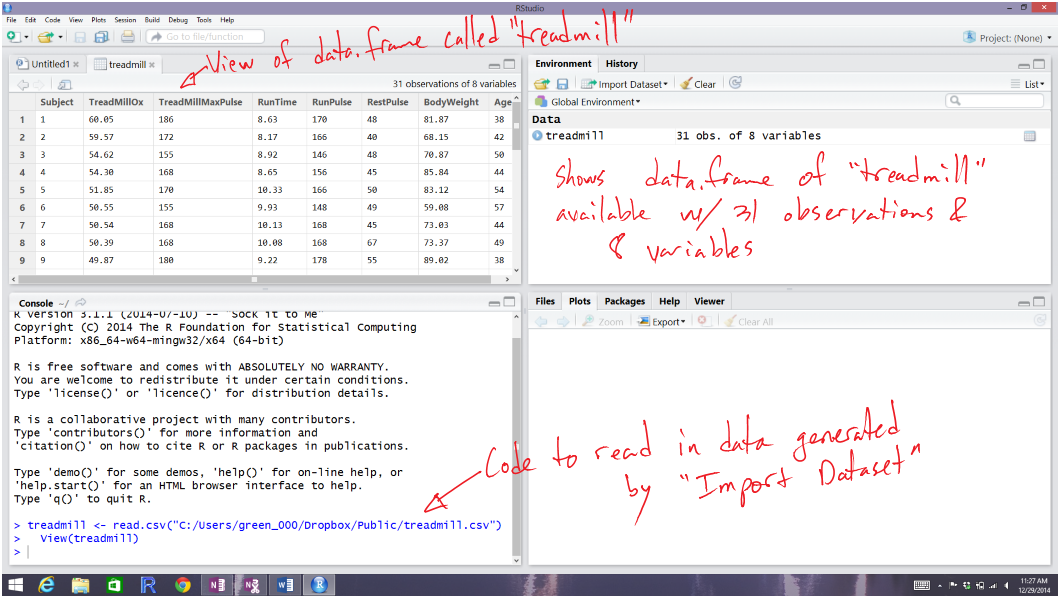
\includegraphics[width=14.72in]{chapter0_files/image005} \caption{RStudio with initial data set loaded}\label{fig:Figure3}
\end{figure}

Just directly typing (or using) a line of code like this is actually the
other way that we can read in files. If you choose to use the text-only
interface, then you need to tell R where to look in your computer to
find the data file. \texttt{read.csv} is a function that takes a path as
an argument. To use it, specify the path to your data file, put quotes
around it, and put it as the input to \texttt{read.csv(...)} . For some
examples later in the book, you will be able to copy a command like this
from the text and read data sets and other code directly from my the
course folder, assuming you are connected to the internet.

To verify that you read the data set in correctly, it is always good to
check its contents. We can view the first and last rows in the data set
using the \texttt{head} and \texttt{tail} functions on the data set,
which show the following results for the \texttt{treadmill} data. Note
that you will sometimes need to resize the console window in RStudio to
get all the columns to display in a single row which can be performed by
dragging the gray bars that separate the panels.

\begin{Shaded}
\begin{Highlighting}[]
\KeywordTok{head}\NormalTok{(treadmill)}
\end{Highlighting}
\end{Shaded}

\begin{verbatim}
##   Subject TreadMillOx TreadMillMaxPulse RunTime RunPulse RestPulse
## 1       1       60.05               186    8.63      170        48
## 2       2       59.57               172    8.17      166        40
## 3       3       54.62               155    8.92      146        48
## 4       4       54.30               168    8.65      156        45
## 5       5       51.85               170   10.33      166        50
## 6       6       50.55               155    9.93      148        49
##   BodyWeight Age
## 1      81.87  38
## 2      68.15  42
## 3      70.87  50
## 4      85.84  44
## 5      83.12  54
## 6      59.08  57
\end{verbatim}

\begin{Shaded}
\begin{Highlighting}[]
\KeywordTok{tail}\NormalTok{(treadmill)}
\end{Highlighting}
\end{Shaded}

\begin{verbatim}
##    Subject TreadMillOx TreadMillMaxPulse RunTime RunPulse RestPulse
## 26      26       44.61               182   11.37      178        62
## 27      27       40.84               172   10.95      168        57
## 28      28       39.44               176   13.08      174        63
## 29      29       39.41               176   12.63      174        58
## 30      30       39.20               172   12.88      168        44
## 31      31       37.39               192   14.03      186        56
##    BodyWeight Age
## 26      89.47  44
## 27      69.63  51
## 28      81.42  44
## 29      73.37  57
## 30      91.63  54
## 31      87.66  45
\end{verbatim}

While not always required, for many of the analyses, we will tap into a
large suite of additional functions available in R packages by
``installing'' (basically downloading) and then ``loading'' the
packages. There are some packages that we will use frequently, starting
with the \texttt{mosaic} package (Pruim, Kaplan, and Horton, tab in the
lower right panel of RStudio. Click on the \textbf{Install} button and
then type in the name of the package in the box (here type in
\texttt{mosaic}). RStudio will try to auto-complete the package name you
are typing which should help you make sure you got it typed correctly.
This will be the first of \emph{many} times that we will mention that R
is case sensitive -- in other words, \texttt{Mosaic} is different from
\texttt{mosaic} in R syntax and this sort of thing applies to everything
you do in R. You should only need to install each R package once on a
given computer. If you ever see a message that R can't find a package,
make sure it appears in the list in the \textbf{Packages} tab and if it
doesn't, repeat the previous steps to install it.

After installing the package, we need to load it to make it active in a
given work session. Go to the command prompt and type (or copy and
paste) \texttt{require(mosaic)} :

\begin{Shaded}
\begin{Highlighting}[]
\KeywordTok{require}\NormalTok{(mosaic)}
\end{Highlighting}
\end{Shaded}

You may see a warning message about versions of the package and versions
of R -- this is \emph{usually} something you can ignore. Other warning
messages could be more ominous for proceeding but before getting too
concerned, there are couple of basic things to check. First, double
check that the package is installed (see previous steps). Second, check
for typographical errors in your code -- especially for mis-spellings or
unintended capitalization. If you are still having issues, try repeating
the installation process. If that fails, find someone more used to using
R to help you (for example in the Math Learning Center or by emailing
your instructor)\footnote{Most computer lab computers at Montana State
  University have RStudio installed and so provide another venue to try
  this where the software is already installed.}.

To help you go from basic to intermediate R usage and especially to help
with more complicated problems, you will want to learn how to manage and
save your R code. The best way to do this is using the upper left panel
in RStudio using what are called R Scripts, which are files that have a
file extension of ``.R''. To start a new ``.R''" file to store your
code, click on \textbf{File} , then \textbf{New File}, then **R Script*.
This will create a blank page to enter and edit code -- then save the
file as MyFileName.R in your preferred location. Saving your code will
mean that you can return to where you last were working by simply
re-running the saved script file. With code in the script window, you
can place the cursor on a line of code or highlight a chunk of code and
hit the ``Run'' button on the upper part of the panel. It will appear in
the console with results just like what you would obtain if you typed it
after the command prompt and hit enter for each line.

Figure \ref{fig:Figure4} shows the screen with the code used in this
section in the upper left panel, saved in file called Ch0.R, with the
results of highlighting and executing the first section of code using
the ``Run'' button.



\begin{figure}
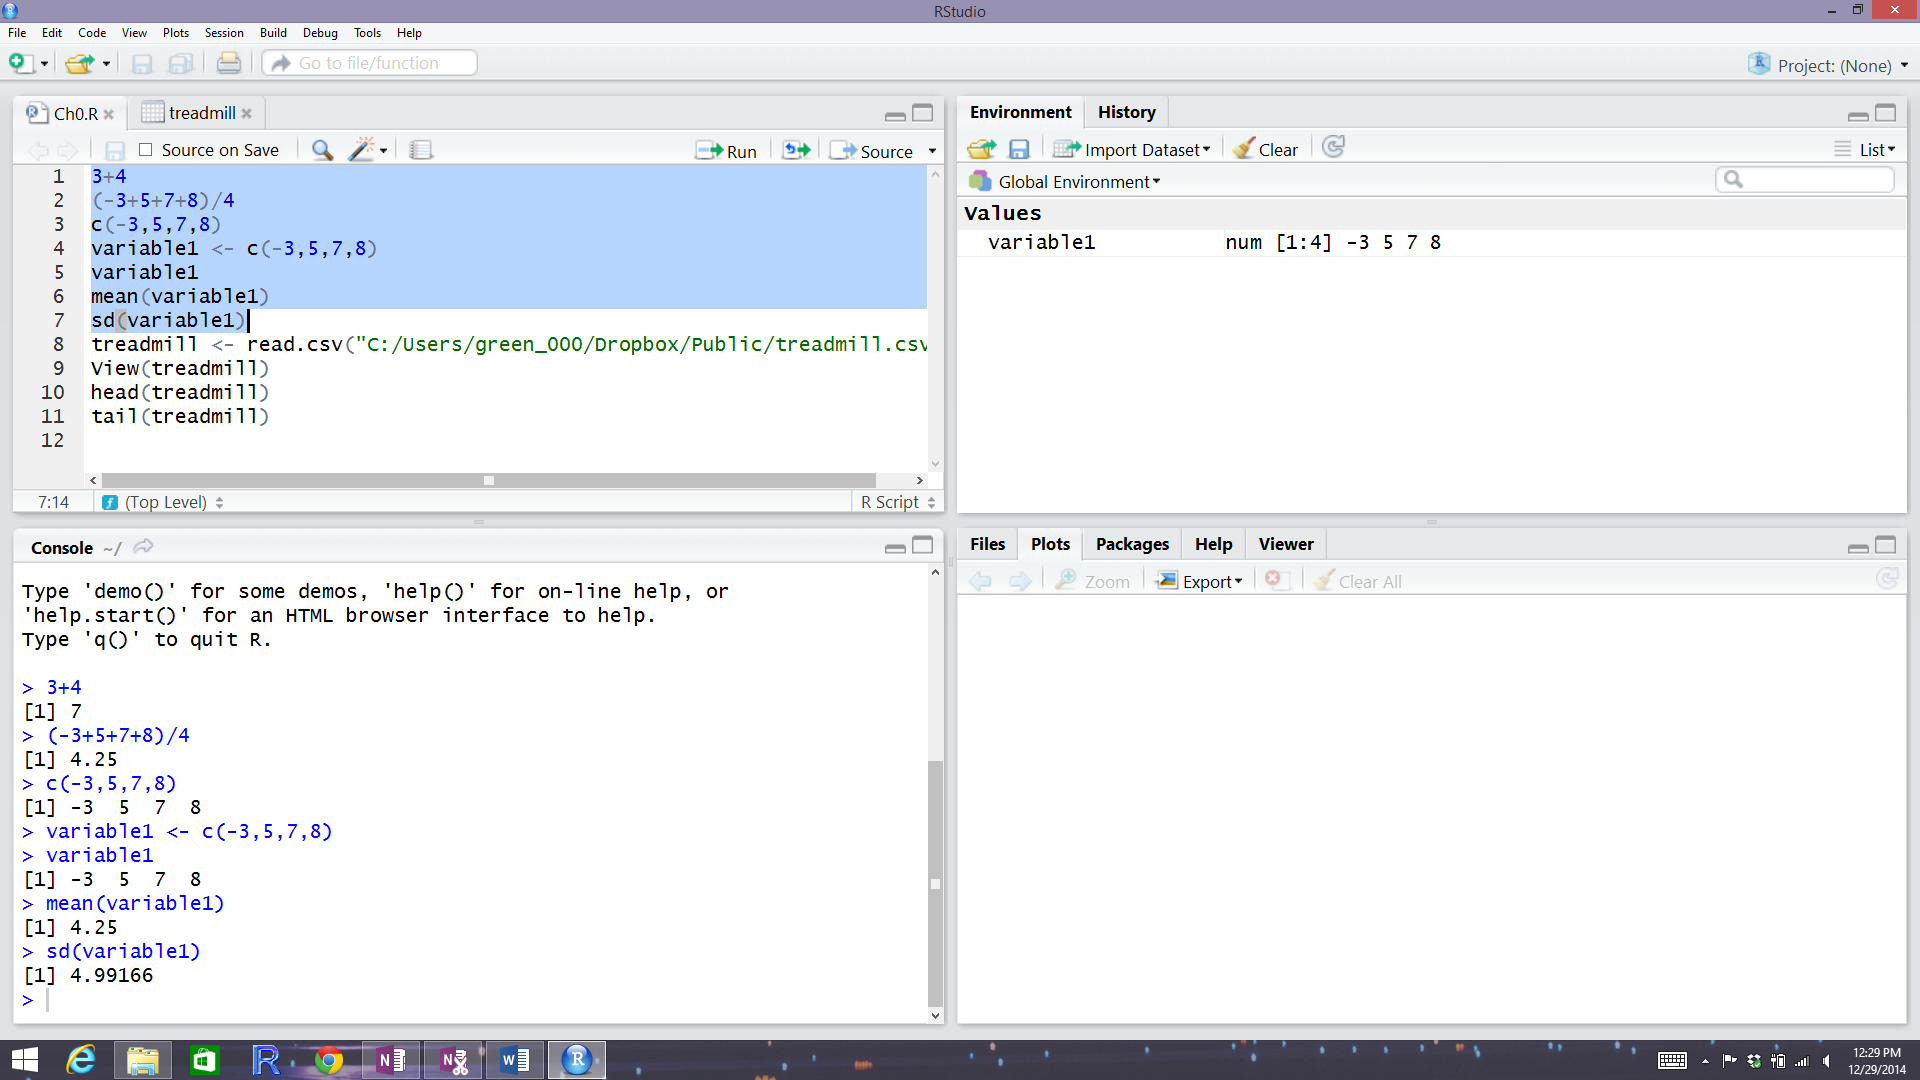
\includegraphics[width=26.67in]{chapter0_files/image006} \caption{RStudio with highlighted code run}\label{fig:Figure4}
\end{figure}

\section{Basic summary statistics, histograms, and boxplots using
R}\label{basic-summary-statistics-histograms-and-boxplots-using-r}

With RStudio running, the \texttt{mosaic} package loaded, a place to
write and save code, and the \texttt{treadmill} data set loaded, we can
(finally!) start to summarize the results of the study. The
\texttt{treadmill} object is what R calls a
\textbf{\emph{data.frame}}\footnote{Data frames in R are objects that
  can contain both categorical and quantitative variables on your n
  subjects with a name for each variable that is also the name of each
  column in a matrix. Each subject is a row of the data set.} and
contains columns corresponding to each variable in the spreadsheet.
Every function in R will involve specifying the variable(s) of interest
and how you want to use them. To access a particular variable (column)
in a data. frame, you can use a \$ between the data. frame name and the
name of the variable of interest, generically as
\texttt{dataframename\$variablename}. To identify the \texttt{RunTime}
variable here it would be \texttt{treadmill\$RunTime}. In the command
line it would look like:

\begin{Shaded}
\begin{Highlighting}[]
\NormalTok{treadmill$RunTime}
\end{Highlighting}
\end{Shaded}

\begin{verbatim}
##  [1]  8.63  8.17  8.92  8.65 10.33  9.93 10.13 10.08  9.22  8.95 10.85
## [12]  9.40 11.50 10.50 10.60 10.25 10.00 11.17 10.47 11.95  9.63 10.07
## [23] 11.08 11.63 11.12 11.37 10.95 13.08 12.63 12.88 14.03
\end{verbatim}

Just as in the previous section, we can generate summary statistics
using functions like \texttt{mean} and \texttt{sd} by running them on a
specific variable:

\begin{Shaded}
\begin{Highlighting}[]
\KeywordTok{mean}\NormalTok{(treadmill$RunTime)}
\end{Highlighting}
\end{Shaded}

\begin{verbatim}
## [1] 10.58613
\end{verbatim}

\begin{Shaded}
\begin{Highlighting}[]
\KeywordTok{sd}\NormalTok{(treadmill$RunTime)}
\end{Highlighting}
\end{Shaded}

\begin{verbatim}
## [1] 1.387414
\end{verbatim}

And now we know that the average running time for 1.5 miles for the
subjects in the study was 10.6 minutes with a standard deviation (SD) of
1.39 minutes. But you should remember that the mean and SD are only
appropriate summaries if the distribution is roughly
\textbf{\emph{symmetric}} (both sides of the distribution are
approximately the same). The \texttt{mosaic} package provides a useful
function called \texttt{favstats} that provides the mean and SD as well
as the \textbf{\emph{5 number summary}} : the minimum (\texttt{min}),
the first quartile (\texttt{Q1}, the 25\(^{th}\) percentile), the median
(50\(^{th}\) percentile), the third quartile (\texttt{Q3} , the
75\(^{th}\) percentile), and the maximum (\texttt{max}). It also
provides the number of observations (\texttt{n}) which was 31, as noted
above, and a count of whether any missing values were encountered
(\texttt{missing}), which was 0 here since all subjects had measurements
available on this variable.

\begin{Shaded}
\begin{Highlighting}[]
\KeywordTok{favstats}\NormalTok{(treadmill$RunTime)}
\end{Highlighting}
\end{Shaded}

\begin{verbatim}
##   min   Q1 median    Q3   max     mean       sd  n missing
##  8.17 9.78  10.47 11.27 14.03 10.58613 1.387414 31       0
\end{verbatim}

We are starting to get somewhere with understanding that the runners
were somewhat fit with worst runner covering 1.5 miles in 14 minutes
(the equivalent of a 9.3 minute mile) and the best running at a 5.4
minute mile pace. The limited variation in the results suggests that the
sample was obtained from a restricted group with somewhat common
characteristics. When you explore the ages and weights of the subjects
in the Practice Problems in Section 0.5, you will get even more
information about how similar all the subjects in this study were.

A graphical display of these results will help us to assess the shape of
the distribution of run times -- including considering the potential for
the presence of a \textbf{\emph{skew}} (whether the right or left tail
of the distribution is noticeably more spread out with left skew meaning
that the left tail is more spread out than the right tail) and
\textbf{\emph{outliers}}\\
(unusual observations). A \textbf{\emph{histogram }} is a good place to
start. Histograms display connected bars with counts of observations
defining the height of bars based on a set of bins of values of the
quantitative variable. We will apply the \texttt{hist} function to the
\texttt{RunTime} variable, which produces Figure \ref{fig:Figure5}.




\begin{Shaded}
\begin{Highlighting}[]
\KeywordTok{hist}\NormalTok{(treadmill$RunTime)}
\end{Highlighting}
\end{Shaded}

\begin{figure}[htbp]
\centering
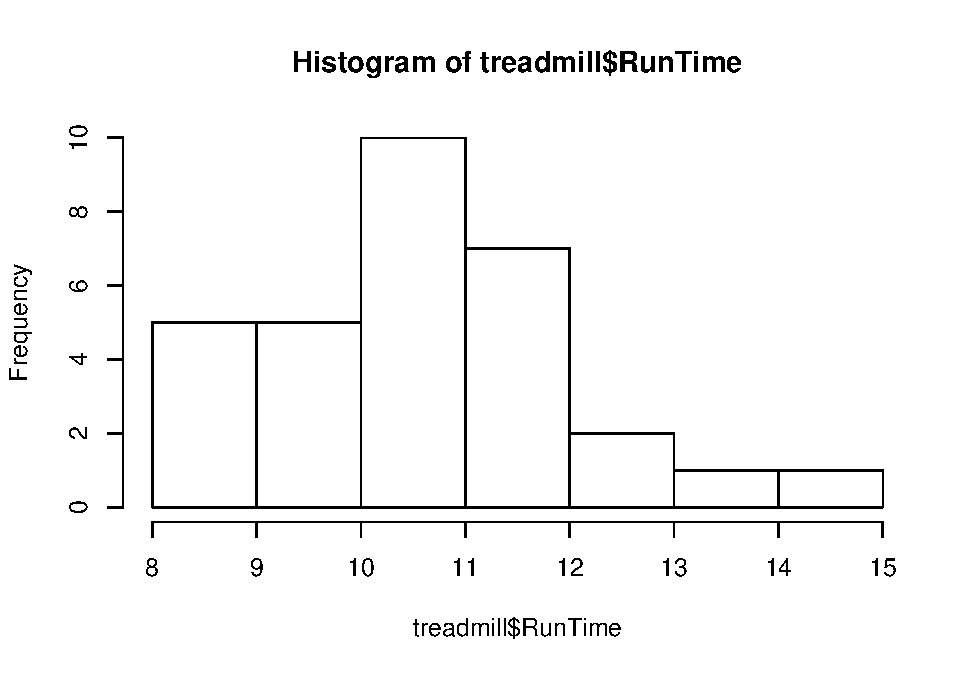
\includegraphics{GreenwoodBanner_files/figure-latex/Figure5-1.pdf}
\caption{\label{fig:Figure5}Histogram of Run Times \#(minutes) of n=31 subjects in
Treadmill study.}
\end{figure}

I used the \textbf{Export} button found above the plot, followed by
\textbf{Copy to Clipboard} and clicking on the \textbf{Copy Plot}
button. Then if you open your favorite word-processing program, you
should be able to paste it into a document for writing reports that
include the figures. You can see the first parts of this process in the
screen grab in Figure \ref{fig:Figure6}.



\begin{figure}
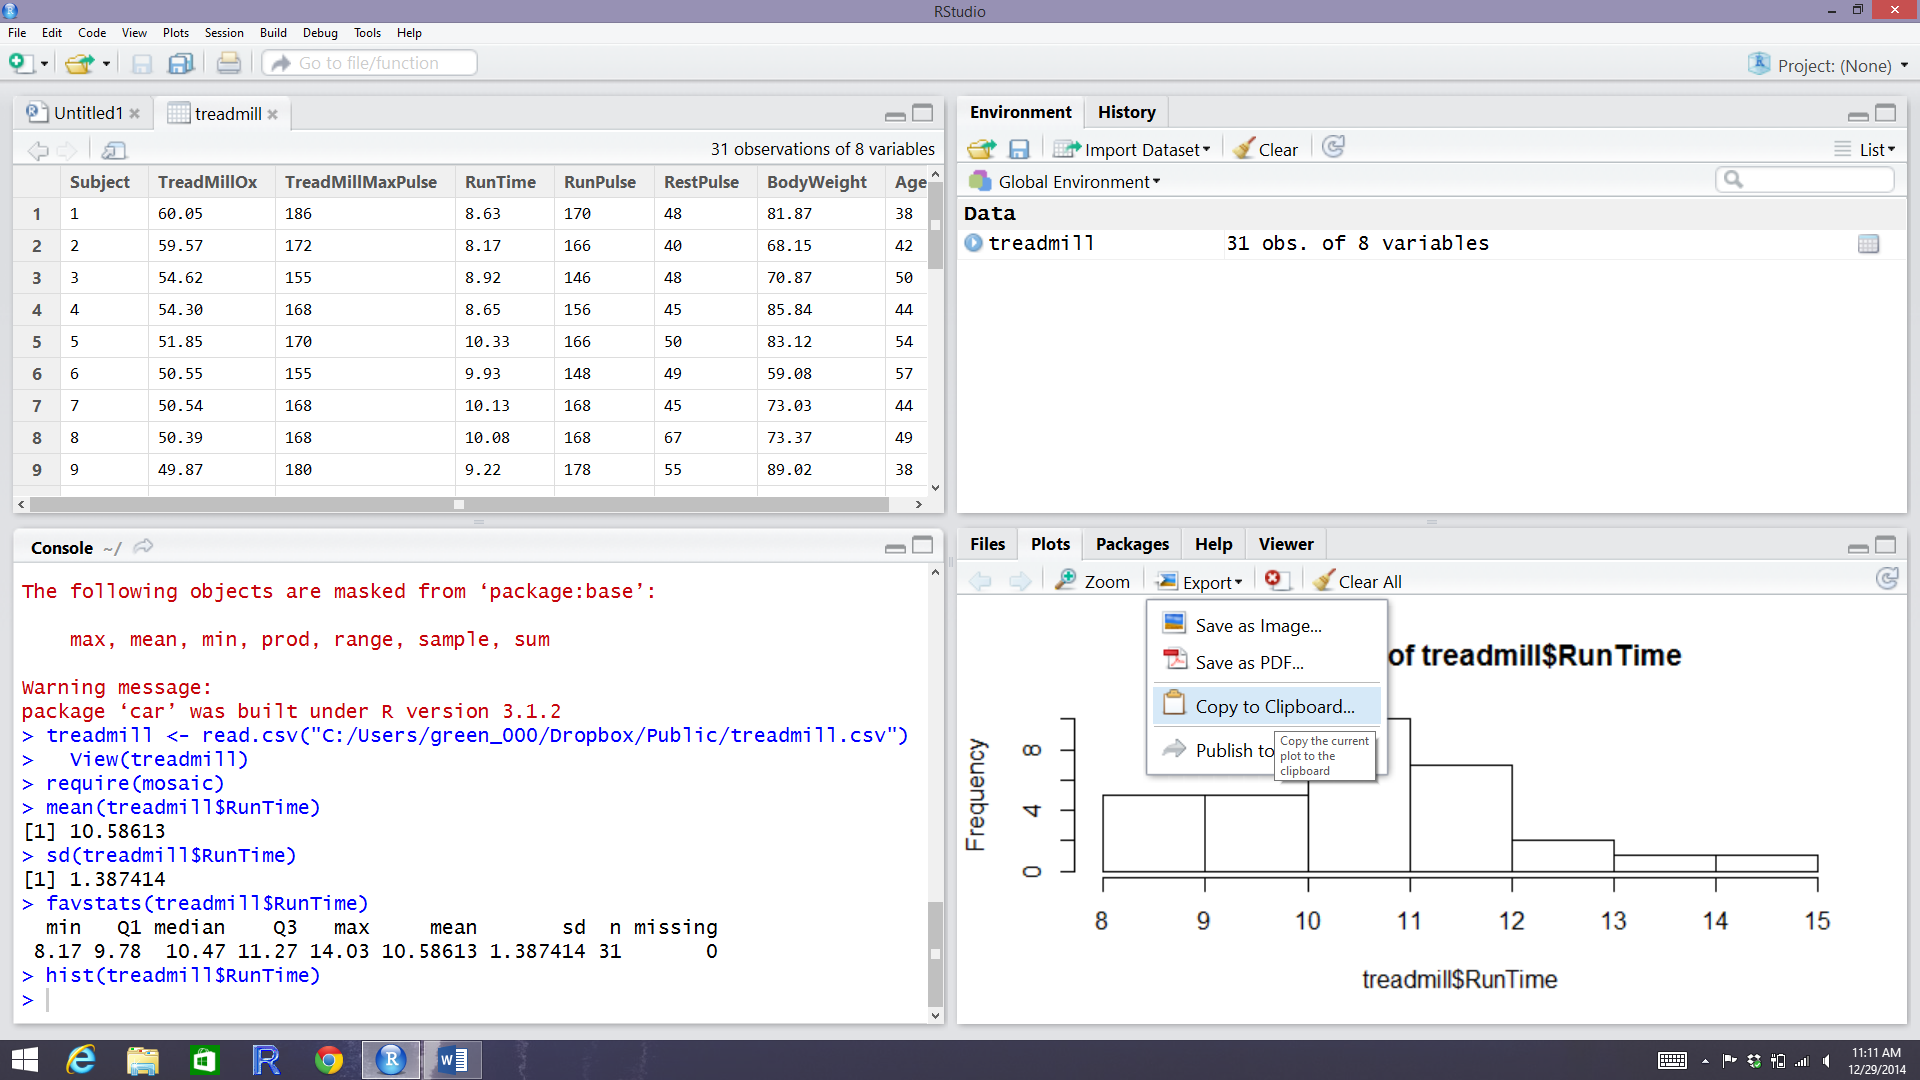
\includegraphics[width=26.67in]{chapter0_files/image010} \caption{RStudio while in the process of copying the histogram}\label{fig:Figure6}
\end{figure}

You can also directly save the figures as separate files using
\textbf{Save as Image} or \textbf{Save as PDF}and then insert them into
your word processing documents.

The function \texttt{hist} defaults into providing a histogram on the
\textbf{\emph{frequency}} (count) scale. In most R functions, there are
the default options that will occur if we don't make any specific
choices but we can override the default options if we desire. One option
we can modify here is to add labels to the bars to be able to see
exactly how many observations fell into each bar. Specifically, we can
turn the \texttt{labels} option ``on'' by making it true (``T'') by
adding \texttt{labels=T} to the previous call to the \texttt{hist}
function, separated by a comma:



\begin{Shaded}
\begin{Highlighting}[]
\KeywordTok{hist}\NormalTok{(treadmill$RunTime, }\DataTypeTok{labels=}\NormalTok{T)}
\end{Highlighting}
\end{Shaded}

\begin{figure}[htbp]
\centering
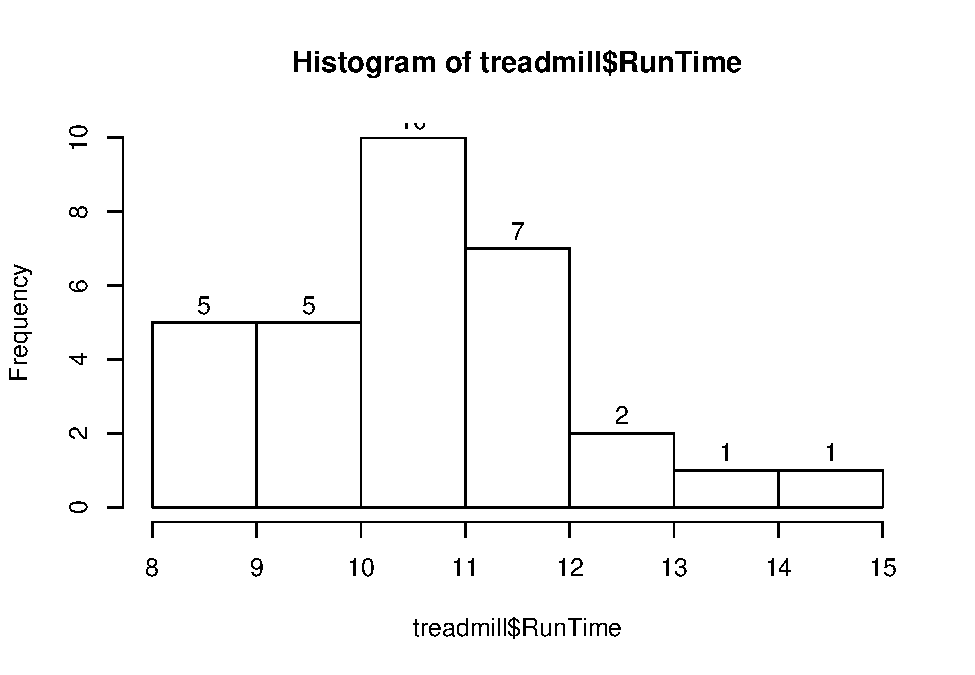
\includegraphics{GreenwoodBanner_files/figure-latex/Figure7-1.pdf}
\caption{\label{fig:Figure7}Histogram of \#Run Times with counts in bars labeled.}
\end{figure}

Based on this histogram, it does not appear that there any outliers in
the responses since there are no bars that are separated from the other
observations. However, the distribution does not look symmetric and
there might be a skew to the distribution. Specifically, it appears to
be \textbf{\emph{skewed right}} (the right tail is longer than the
left). But histograms can sometimes mask features of the data set by
binning observations and it is hard to find the percentiles accurately
from the plot.

When assessing outliers and skew, the \textbf{\emph{boxplot}}\\
(or \emph{Box and Whiskers} plot) can also be helpful (Figure
\ref{fig:Figure8}) to describe the shape of the distribution as it
displays the 5-number summary and will also indicate observations that
are ``far'' above the middle of the observations. R's \texttt{boxplot}
function uses the standard rule to indicate an observation as a
\textbf{\emph{potential outlier}} if it falls more than 1.5 times the
\textbf{\emph{IQR}} (Inter-Quartile Range, calculated as Q3-Q1) below Q1
or above Q3. The potential outliers are plotted with circles and the
\emph{Whiskers} (lines that extend from Q1 and Q3 typically to the
minimum and maximum) are shortened to only go as far as observations
that are within \(1.5*\)IQR of the upper and lower quartiles. The
\emph{box} part of the boxplot is a box that goes from Q1 to Q3 and the
median is displayed as a line somewhere inside the box\footnote{The
  median, quartiles and whiskers sometimes occur at the same values when
  there are many tied observations. If you can't see all the components
  of the boxplot, produce the numerical summary to help you understand
  what happened.}. Looking back at the summary statistics above, Q1=9.78
and Q3=11.27, providing an IQR of:

\begin{Shaded}
\begin{Highlighting}[]
\NormalTok{IQR <-}\StringTok{ }\FloatTok{11.27} \NormalTok{-}\StringTok{ }\FloatTok{9.78}
\end{Highlighting}
\end{Shaded}

One observation (the maximum value of 14.03) is indicated as a potential
outlier based on this result by being larger than Q3 \(+1.5*\)IQR, which
was 13.505:

\begin{Shaded}
\begin{Highlighting}[]
\FloatTok{11.27} \NormalTok{+}\StringTok{ }\FloatTok{1.5}\NormalTok{*IQR}
\end{Highlighting}
\end{Shaded}

\begin{verbatim}
## [1] 13.505
\end{verbatim}

The boxplot also shows a slight indication of a right skew (skew towards
larger values) with the distance from the minimum to the median being
smaller than the distance from the median to the maximum. Additionally,
the distance from Q1 to the median is smaller than the distance from the
median to Q3. It is modest skew, but worth noting.



\begin{Shaded}
\begin{Highlighting}[]
\KeywordTok{boxplot}\NormalTok{(treadmill$RunTime)}
\end{Highlighting}
\end{Shaded}

\begin{figure}[htbp]
\centering
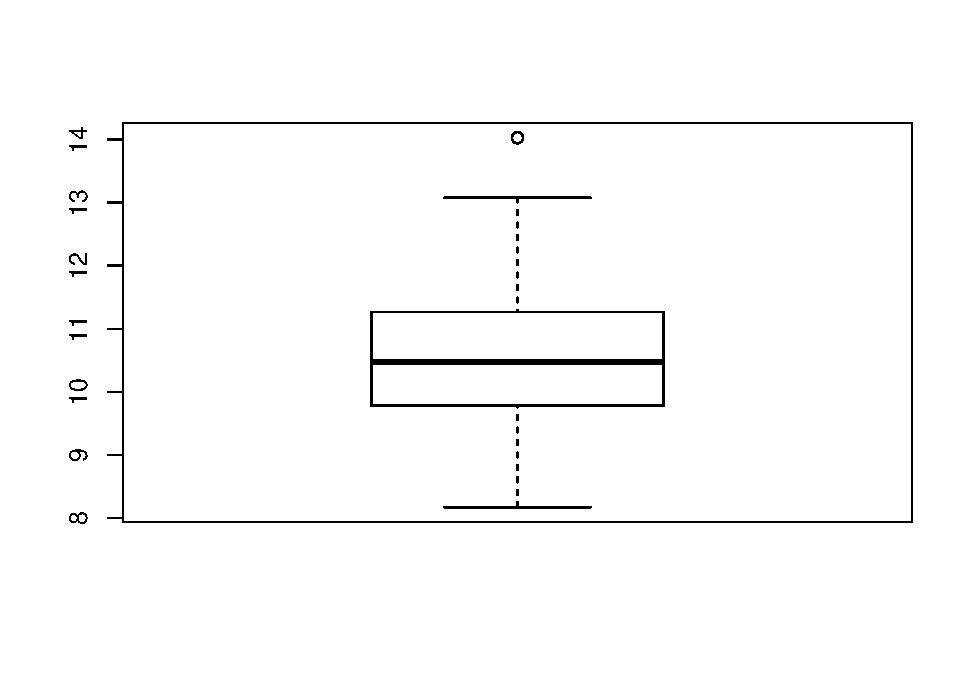
\includegraphics{GreenwoodBanner_files/figure-latex/Figure8-1.pdf}
\caption{\label{fig:Figure8}Boxplot of 1.5 mile Run Times.}
\end{figure}

While the default boxplot is fine, it fails to provide good graphical
labels, especially on the y-axis. Additionally, there is no title on the
plot. The following code provides some enhancements to the plot by using
the \texttt{ylab} and \texttt{main} options in the call to
\texttt{boxplot}, with the results displayed in Figure
\ref{fig:Figure9}. When we add text to plots, it will be contained
within quotes and be assigned into the options \texttt{ylab} (for
y-axis) or \texttt{main} (for the title) here to put it into those
locations.



\begin{Shaded}
\begin{Highlighting}[]
\KeywordTok{boxplot}\NormalTok{(treadmill$RunTime, }\DataTypeTok{ylab=}\StringTok{"1.5 Mile Run Time (minutes)"}\NormalTok{, }
        \DataTypeTok{main=}\StringTok{"Boxplot of the Run Times of n=31 participants"}\NormalTok{)}
\end{Highlighting}
\end{Shaded}

\begin{figure}[htbp]
\centering
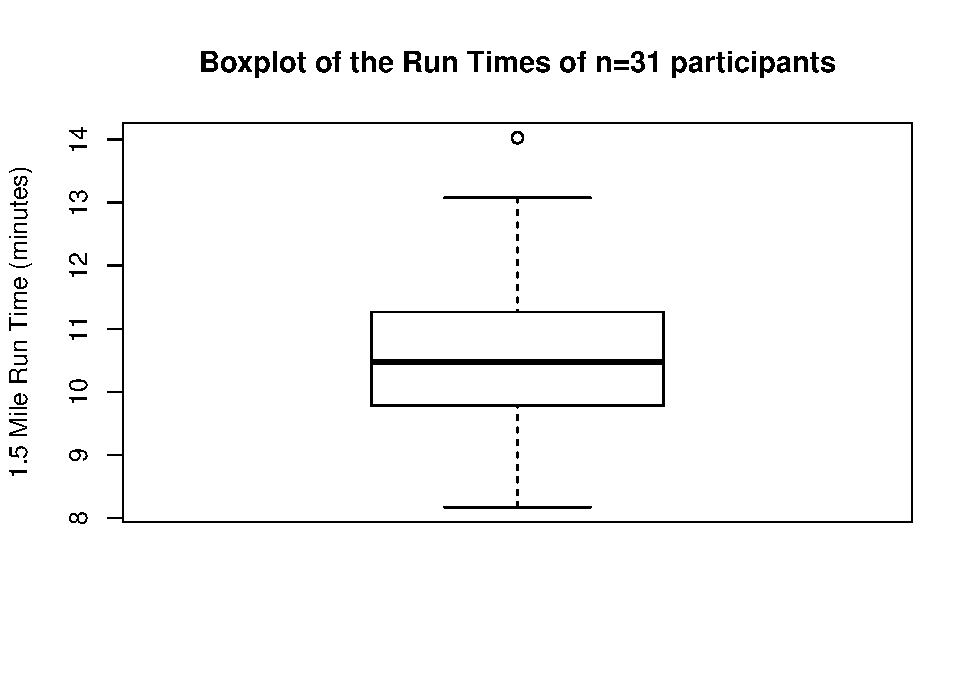
\includegraphics{GreenwoodBanner_files/figure-latex/Figure9-1.pdf}
\caption{\label{fig:Figure9}Boxplot of Run Times with improved labels.}
\end{figure}

Throughout the book, we will often use extra options to make figures
that are easier for you to understand. There are often simpler versions
of the functions that will suffice but the extra work to get better
labeled figures is often worth it. I guess the point is that ``a picture
is worth a thousand words'' but in data visualization, that is only true
if the reader can understand what is being displayed. It is also
important to think about the quality of the information that is being
displayed, regardless of how pretty the graphic might be.

All the previous results were created by running the R code and then
``grabbing'' the results from either the console or by copying the
figure. There is another way to use RStudio where you can have it
compile the results (both output and figures) directly into a document
together with the code that generated it, using what is called RMarkdown
(\url{http://shiny.rstudio.com/articles/rmarkdown.html}). It adds some
additional setup complexity we want to avoid for now but is what we used
to do all the analyses that follow in the book. The main reason to
mention this is that you will see a change in formatting of the R code
and output from here forward as you will no longer see the command
prompt (``\textgreater{}'') with the code. The output will be flagged by
having two ``\#\#'''s before it. For example, the summary statistics for
the \emph{RunTime} variable from `\texttt{favstats} function would look
like:

\begin{Shaded}
\begin{Highlighting}[]
\KeywordTok{favstats}\NormalTok{(treadmill$RunTime)}
\end{Highlighting}
\end{Shaded}

\begin{verbatim}
##   min   Q1 median    Q3   max     mean       sd  n missing
##  8.17 9.78  10.47 11.27 14.03 10.58613 1.387414 31       0
\end{verbatim}

Statisticians (and other scientists) are starting to use these methods
because they provide what is called ``Reproducible research'' (Gandrud,
2015) where all the code and output it produced are available in a
single place. This allows different researchers to run and verify
results or the original researchers to revisit their earlier work at a
later date and recreate all their results. Scientific publications are
currently encouraging researchers to work in this way and may someday
require it. In this book, we focus on the R code and show the results
from running it, but you may want to consider exploring these
alternative options.

Finally, when you are done with your work and attempt to exit out of
RStudio, it will ask you to save your workspace. You do not need to do
this and would be better served not to do this. If you are in the
practice of saving your workspace, you will end up with tons of data.
frames that open each time you use it and it will be harder to find and
manage the ones you are currently working with. If you save your R code
via the script window, you can re-create any results by simply
re-running that code. If you find that you have lots of ``stuff'' in
your workspace, just run \texttt{rm(list\ =\ ls())}. It will delete all
the data sets from your workspace.

\section{Chapter summary}\label{chapter-summary}

This chapter covered getting R and RStudio downloaded and some basics of
working with R via RStudio. You should be able to read a data set into R
and run some basic functions, all done using the RStudio interface. If
you are struggling with this, you should seek additional help with these
technical issues so that you are ready for more complicated statistical
methods that are going to be encountered in the following chapters. For
most assignments, we will give you a seed of the basic R code that you
need and then you will modify it to work on your data set of interest.
As mentioned previously, the way everyone learns R is by starting with
some example code that does most of what you want to do and then you
modify it. If you can complete the Practice Problems that follow, you
are well on your way to learning to use R.

The statistical methods in this chapter were minimal and all should have
been review. They involved a quick reminder of summarizing the center,
spread, and shape of distributions using numerical summaries of the mean
and SD and/or the min, Q1, median, Q3, and max and the histogram and
boxplot as graphical summaries. We revisited the ideas of symmetry and
skew. But the main point was really to get a start on using R to provide
results you should be familiar with from your previous statistics
experience(s).

\section{Important R Code}\label{important-r-code}

To help you learn and use R, there is a section highlighting the most
important R code used near the end of each chapter. The dark text will
never change but the lighter (red) text will need to be customized to
your particular application. The sub-bullet for each function will
discuss the use of the function and pertinent options or packages
required. You can use this as a guide to finding the function names and
some hints about options that will help you to get the code to work or
you can revisit the worked examples using each of the functions.

\begin{itemize}
\item
  FILENAME
  \texttt{\textless{}-\ read.csv("path\ to\ csv\ file/FILENAME.csv")}

  \begin{itemize}
  \tightlist
  \item
    Can be generated using ``Import Dataset'' button or by modifying
    this text.
  \end{itemize}
\item
  DATASETNAME \texttt{\$}VARIABLENAME

  \begin{itemize}
  \tightlist
  \item
    To access a particular variable in a data. frame called DATASETNAME,
    use a \$ and then the VARIABLENAME.
  \end{itemize}
\item
  \texttt{head(}DATASETNAME\texttt{)}

  \begin{itemize}
  \tightlist
  \item
    Provides a list of the first few rows of the data set for all the
    variables in it.
  \end{itemize}
\item
  \texttt{mean(}DATASETNAME\texttt{\$}VARIABLENAME\texttt{)}

  \begin{itemize}
  \tightlist
  \item
    Calculates the mean of the observations in a variable.
  \end{itemize}
\item
  \texttt{sd(}DATASETNAME\texttt{\$}VARIABLENAME\texttt{)}

  \begin{itemize}
  \tightlist
  \item
    Calculates the SD of the observations in a variable.
  \end{itemize}
\item
  \texttt{favstats(}DATASETNAME\texttt{\$}VARIABLENAME\texttt{)}

  \begin{itemize}
  \item
    Provides a suite of numerical summaries of the observations in a
    variable.
  \item
    Requires the package to be loaded (\texttt{require(mosaic}) after
    installing the package).
  \end{itemize}
\item
  \texttt{hist(}DATASETNAME\texttt{\$}VARIABLENAME\texttt{)}

  \begin{itemize}
  \tightlist
  \item
    Makes a histogram.
  \end{itemize}
\item
  \texttt{boxplot(}DATASETNAME\texttt{\$}VARIABLENAME\texttt{)}

  \begin{itemize}
  \tightlist
  \item
    Makes a boxplot.
  \end{itemize}
\end{itemize}

\section{Practice problems}\label{practice-problems}

In each chapter, the last section contains some questions for you to
complete to make sure you understood the material. You can download the
code to answer questions 0.1 to 0.5 below at
\url{http://www.math.montana.edu/courses/s217/documents/Ch0.Rmd}. But to
practice learning R, it would be most useful for you to try to
accomplish the requested tasks yourself and then only refer to the
provided R code if/when you struggle. These questions provide a great
venue to check your learning, often to see the methods applied to
another data set, and for something to discuss in study groups, with
your instructor, and/or at the Math Learning Center.

0.1. Read in the treadmill data set discussed above and find the mean
and SD of the Ages (\emph{Age} variable) and Body Weights
(\emph{BodyWeight} variable). In studies involving human subjects, it is
common to report a summary of characteristics of the subjects. Why does
this matter? Think about how your interpretation of any study of the
fitness of subjects would change if the mean age had been 20 years older
or 35 years younger.

0.2. How does knowing about the distribution of results for \emph{Age}
and \emph{BodyWeight} help you understand the results for the Run Times
discussed above?

0.3. The mean and SD are most useful as summary statistics only if the
distribution is relatively symmetric. Make a discuss the shape of the
distribution (is it skewed right, skewed left, approximately symmetric?;
are there outliers?). Approximately what range of ages does this study
pertain to?

0.4. The weight responses are in kilograms and you might prefer to see
them in pounds. The conversion is lbs=2. 205\emph{kgs. Create a new
variable in the \texttt{treadmill}\\
data.frame called }BWlb* using this code:

\texttt{treadmill\$BWlb\ \textless{}-\ 2.\ 205*treadmill\$BodyWeight}

and find the mean and SD of the new variable (\emph{BWlb}).

0.5. Make histograms and boxplots of the original \emph{BodyWeight} and
new \emph{BWlb} variables. Discuss aspects of the distributions that
changed and those that remained the same with the transformation from
kilograms to pounds.

\chapter{Placeholder}\label{placeholder}

\bibliography{packages,book}


\end{document}
